\section*{Planilla Resumen de Datos de la Propuesta – TEG}

\subsection*{Tema Propuesto:}

\begin{figure}[h]
  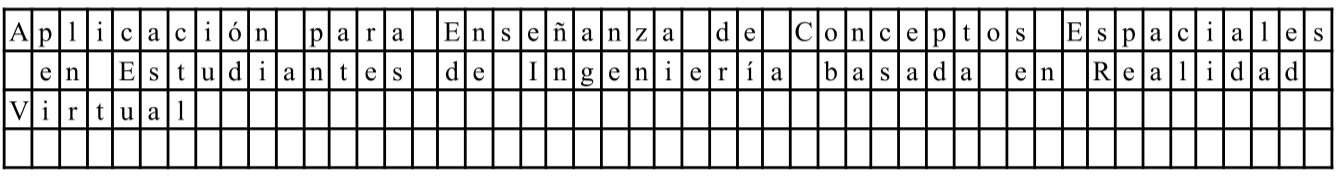
\includegraphics[width=\textwidth]{nombre-04-24.png}
\end{figure}

\subsection*{Datos del Estudiante:}
\begin{table}[h]
  \doublespacing
  \begin{tabularx}{\textwidth}{X c c c}
    \hline
    \textbf{Apellidos, Nombres} & \textbf{C.I.N.}    & \textbf{Teléfono} & \textbf{e-mail}  \\
    \hline
    \small{\estudiante}         & \small{28.031.941} & \small{Insertar}  & \small{Insertar} \\
    \hline
  \end{tabularx}
\end{table}

\subsection*{Datos del Tutor Académico:}

\begin{table}[h]
  \onehalfspacing
  \begin{tabularx}{\textwidth}{>{\hsize=.3\hsize}X X}
    Nombre                       & \academicTutor                                                                       \\
    C.I.N.                       & Insertar                                                                             \\
    Profesión                    & Insertar                                                                             \\
    Años Experiencia Profesional & Insertar                                                                             \\
    Cargo Actual                 & Insertar                                                                             \\
    E-mail                       & Insertar                                                                             \\
    Teléfonos                    & Insertar \tab Oficina: Insertar                                                      \\
    \hline
    Años de Graduado             &
    Insertar \tab[4cm] Tutor TG \hfill Sí \space\fbox{$\checkmark$} \hfill No \space\fbox{\phantom{a}}                  \\
    \hline
    Profesor UCAB                & Sí \space\fbox{$\checkmark$} No \space\fbox{\phantom{a}} \tab[2cm] Escuela: Insertar \\
  \end{tabularx}
\end{table}

\clearpage
